\documentclass[letterpaper]{article}
\usepackage[utf8]{inputenc}
\usepackage[spanish]{babel}
\usepackage{amssymb, amsmath}
\usepackage{graphicx}
\usepackage{lipsum}
\usepackage{dsfont}
\usepackage[margin=1.5cm,
vmargin={1.5cm,1.3cm},
includefoot]{geometry}
\usepackage{setspace}
\usepackage{subcaption}
\usepackage{tocloft}
\usepackage{upgreek}
\usepackage{amsthm}
\usepackage{graphicx}
\usepackage{paralist}
\usepackage{fancyhdr}
\usepackage{lmodern}
\usepackage{tcolorbox}
\usepackage{color}
\usepackage{tikz}
\tcbuselibrary{skins,breakable}
\pagestyle{fancy}

\renewcommand{\headrulewidth}{0.4pt}
\renewcommand{\footrulewidth}{0.4pt}

\providecommand{\abs}[1]{\lvert#1\rvert}
\providecommand{\norm}[1]{\lVert#1\rVert}														  
\providecommand{\pint}[1]{<#1>}														  
\newcommand{\V}{\mathds{V}}

\newcommand{\W}{\mathds{W}}

\newcommand{\F}{\mathds{F}}

\newcommand{\tq}{ \quad \cdot  \backepsilon \cdot \quad }

\newcommand{\ld}{\lim\limits_{x \to 0^{+}}}

\newcommand{\li}{\lim\limits_{x \to 0^{-}}}

\newcommand{\la}{\lim\limits_{x \to a}}

\newcommand{\R}{\mathds{R}}

\renewcommand{\u}{\vec{u}}

\renewcommand{\v}{\vec{v}}

\newcommand{\Po}{\mathds{P}_2(\mathds{R})}

\renewcommand{\*}{\cdot}

\newcommand{\Iden}{\begin{pmatrix}
		1 & 0 & 0\\
		0 & 1 & 0\\
		0 & 0 & 1 
\end{pmatrix}}
\newcommand{\T}{\begin{pmatrix}
		1 & 3 & 9 \\
		1 & 3 & 4 \\
		0 & 0 & 2 
\end{pmatrix} }

\makeatletter
\renewcommand*\env@matrix[1][*\c@MaxMatrixCols c]{%
	\hskip -\arraycolsep
	\let\@ifnextchar\new@ifnextchar
	\array{#1}}
\makeatother

\newtheorem{theorem}{Teorema}[section]
\theoremstyle{definition}
\newtheorem{definition}{Definición}
\begin{document}
	
	\setlength{\unitlength}{1cm}
	\thispagestyle{empty}
	\begin{picture}(19,3)
	\put(-0.5,1.2){
\includegraphics[scale=.20]{unam1.png}}
	\put(16,1){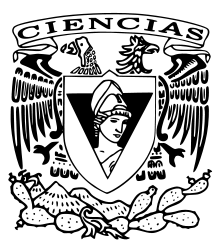
\includegraphics[scale=.29]{fciencias1.png}}
	\end{picture}
	
	\begin{center}
		\vspace{-114pt}
		\textbf{\large Matemáticas para las Ciencias II}\\
		\textbf{ Semestre 2020-2}\\
		Prof. Pedro Porras Flores\\
		Ayud. Irving Hernández Rosas \\
		\textbf{Tarea-examen I}\\[0.2cm]
		Kevin Ariel Merino Peña\footnote{317031326}\\ [0.2cm]
	\end{center}
	\vspace{-10pt}
	\rule{19cm}{0.3mm}
	
\section[Clase 23 de marzo]{Conjuntos abiertos}
\begin{theorem}
	Sean $ \vec{u} $ y $ \vec{v} $ dos vectores en $ \R^3 $ y sea $ \theta  \in \R$, donde $ 0 \leq \theta < \pi $ el ángulo entre ellos, entonces
	\[ <\vec{u}, \vec{v}> = \norm{\vec{u}}\norm{\vec{v}}\cos \theta \]
\end{theorem}
\begin{proof}
	Consideremos el triángulo formado por los vectores $ \vec{u}, \vec{v} $ y $ \vec{u}\vec{v} $ de la ley de cosenos tenemos 
	\[ \norm{\vec{u}- \vec{v}}^2 = \norm{\vec{u}}^2 + \norm{\vec{v}}^2 - 2 \norm{\vec{u}}\norm{\vec{v}}\cos\theta \]
	Por otro lado calculemos $ \norm{\vec{u} - \vec{v}}^2 $ esto es
	\begin{align*}
		\norm{\vec{u}- \vec{v}}^2 &= \pint{\u - \v, \u - \v} \\
		\norm{\vec{u}- \vec{v}}^2 &= \pint{\u, \u - \v} + \pint{-\v, \u - \v} \\
		\norm{\vec{u}- \vec{v}}^2 &= \pint{\u, \u - \v} + \pint{-\v, \u - \v} \\
	\end{align*}
\end{proof}
\end{document}